% !TEX root =  master.tex
\chapter{Umsetzung} \label{umsetzung}
	\section[Organisation]{Organisation{\hfill \normalsize Sandra Keller}}
	GitHub
	\section[Backend]{Backend{\hfill \normalsize Martin Sandig}}
\subsection{Grundgerüst}\label{umsetzung:backend:grundgeruest}
--> Komponentendiagramm erstellen

Das Backend wurde anhand des Fachkonzeptes implementiert. Da die grundlegende Anforderung für dieses, die Umsetzung in Java ist, wurde hierzu ein Java-Projekt mit Maven aufgesetzt. Apache Maven ist ein Software-Projektmanagement- und Verständniswerkzeug.\autocite{ApacheSoftwareFoundation} Es dient unter anderem dazu den Aufbau von Projekten zu definieren, benutzte Frameworks zentral zu organisieren sowie einen Projektlebenszyklus abzubilden. Der in Maven implementierte Lebenszyklus umfasst mehrere Stadien, welche sich vom \glqq Clean\grqq, also dem Aufräumen eines Projektes, über \glqq Test\grqq \, bis zum \glqq Install\grqq \, bzw. \glqq Deploy\grqq \, erstrecken. Zwischen diesen Stadien existieren noch viele mehr, welche für diese Seminararbeit keine Rolle spielen sollen. Am Ende des \glqq Install\grqq -Stadiums steht eine ausführbare JAR-Datei zur Verfügung.

Die Konfiguration von Maven wird in einem \ac{POM} definiert. Hierzu existiert eine \glqq pom.xml\grqq-Datei im \ac{ICS}-Projekt. Die eigentliche Umsetzung des Backendes erfolgte mit Hilfe des \glqq Spring\grqq -Frameworks. Spring ist ein Framework, welches für die Entwicklung von Java-Projekten vereinfachen soll sowie ein breites Spektrum an Funktionalitäten für Geschäftslogiken mitliefert.  Genauer gesagt beruht das Backend auf \glqq Spring-Boot\grqq, welches ein Bestandteil des Spring-Frameworks ist. Es dient dazu eigenständig lauffähige Spring-Anwendungen zu entwickeln, wobei alle nötigen Bibliotheken mitgeliefert werden.\autocite{PivotalSoftwareInc} In diesem Fall handelt es sich um eine Spring-Boot-Webanwendung. Für die Konfiguration des \ac{POM} gibt es vordefinierte Templates, sogennante \glqq Archetypes\grqq. Aus diesen heraus lässt sich ein Maven-Projekt generieren, welches alle nötigen Basiseinstellungen mitbringt. Einen solcher \glqq Archetype\grqq \, existiert auch für Spring-Boot-Anwendungen, welcher für das \ac{ICS}-Projekt genutzt wurde.

Das Spring-Framework arbeitet mit Hilfe von \ac{IoC}-Containern. \ac{IoC} ist ein Prinzip bei der Software-Entwicklung, bei der man die Steuerung der Anwendung bzw. die Steuerung von Objekten auf einen Container bzw. an ein Framework übertragen wird. Die \ac{IoC}-Container im Spring-Framework arbeiten nach dem \ac{DI}-Konzept, bei dem Abhängigkeiten von Objekten behandelt werden. Durch dieses Konzept müssen Objekte ihrer Abhängigkeiten nicht selber suchen sondern bekommen die benötigten Ressourcen bzw. Abhängigkeitsobjekte vom Framework zugewiesen. (QUELLE) Der \ac{IoC}-Container, welcher in diesem Projekt genutzt wurde nennt sich \glqq Application-Context \grqq. Objekte, welche sich in diesem Container bzw. Kontext befinden werden \glqq Spring Beans\grqq \, genannt. Spring Beans können auf verschiedene Arten deklariert und initiiert werden. Im Fall dieses Projektes werden alle benötigten Spring Beans beim Starten der Anwendung initiiert. Die Deklaration der Beans erfolgt zum einen durch Java-Annotations innerhalb von Java-Klassen. Zum Anderen werden die Beans in einer Konfigurationsdatei des Application-Contextes definiert. Diese Datei nennt sich \glqq applicationContext.xml\grqq.

Um nun die Spring-Boot-Anwendung ausführbar zu machen wurden zwei Klassen, siehe Quelltext \ref{lst:IcsApplication} und \ref{lst:IcsWebConfiguration} angelegt. Innerhalb der IcsApplication-Klasse wird mit Hilfe der Annotation \glqq @SpringBootApplication\grqq \, und dem Inhalt der \glqq main-Methode\grqq \, definiert, dass es sich um eine Spring-Boot-Anwendung handelt. Die Klasse \glqq IcsWebConfiguration\grqq \, dient zur erweiterten Konfiguration der Spring-Boot-Anwendung. Durch die Annotation \glqq @Configuration\grqq \, und die Implementierung des \glqq WebMvcConfigurer\grqq \, wird dem Spring-Framework mitgeteilt, dass es sich hierbei um eine Konfigurationsklasse handelt, welche beim Starten der Anwendung berücksichtigt werden muss. Durch die Annotation \glqq @ImportResource(...)\grqq \, wird die Konfigurationsdatei für den Application-Context geladen.

\lstset{language=Java}
\begin{lstlisting}[caption={IcsApplication.java}, label={lst:IcsApplication}]
@SpringBootApplication
@EnableAutoConfiguration
@EnableScheduling
public class IcsApplication {
public static void main(String[] args) {
SpringApplication.run(IcsApplication.class, args);
}
}
\end{lstlisting}

\lstset{language=Java}
\begin{lstlisting}[caption={IcsWebConfiguration.java}, label={lst:IcsWebConfiguration}]
@Configuration
@ImportResource("classpath:spring/applicationContext.xml")
public class IcsWebConfiguration implements WebMvcConfigurer {
/**Something more **/
@Override
public void addResourceHandlers(ResourceHandlerRegistry registry) {
if (System.getProperty("os.name").contains("Windows")) {
registry
.addResourceHandler("/content/**")
.addResourceLocations("file:///".concat(
ApplicationEnvironment.getContentPath()
.toString().concat("/")));
} else {
registry
.addResourceHandler("/content/**")
.addResourceLocations("file://".concat(
ApplicationEnvironment.getContentPath()
.toString().concat("/")));
}
}
}
\end{lstlisting}

Da es sich beim \ac{ICS}-Projekt um eine Webanwendung handelt wurde in der \glqq IcsWebConfiguration \grqq -Klasse, siehe Quelltext \ref{lst:IcsWebConfiguration}, ein weiterer \glqq ResourceHandler\grqq \, hinzugefügt, welcher einen \glqq content\grqq-Ordner auf dem Dateisystem zu einer URL (\glqq localhost:8080/content/*\grqq) der Webanwendung zuordnet. Dieser Ordner dient als Ablage für anzuzeigende Bilder der späteren Webseite. Damit dieser Ordner auf dem Dateisystem vorhanden ist, wurde ein Klasse \glqq FileSystemInitilizer\grqq implementiert. Beim Start der Anwendung wird ein Spring-Bean dieser Klasse initiiert, welches eine Ordnerstruktur auf dem Dateisystem anlegt. Hierfür ist es möglich eine Umgebungsvariable für die Anwendung zu setzten. Sollte diese nicht gesetzt worden sein, wird stattdessen der \glqq tmp\grqq- Ordner auf dem Root-Verzeichnis des Betriebssystems als Ausgangsordner für die Dateistruktur der Anwendung verwendet.


\subsection{Datenbank}
\subsubsection{Technologie}
Für die \ac{ICS}-Anwendung wurde beschlossen eine Datenbank als Persistenz-Schicht zu verwenden. Das Schema dieser wurde anhand des ER-Modells aus der Entwurfsphase (ER DIA!!!!) entwickelt. Hierzu wurde ein Java-Framework namens \glqq Liquibase\grqq \, verwendet.\autocite{Liquibase} Liquibase ist ein Framework zum Verfolgen, Verwalten und Anwenden von Datenbankschemaänderungen, welches unabhängig von der zugrundeliegenden Datenbank arbeitet. Das Framework arbeitet mit einem sogenannten \glqq Database-Changelog \grqq, in welchem die Änderungshistorie des Datenbankschemas festgehalten wird. Der Changelog wird in einer XML-Struktur festgehalten. Diese Änderungshistorie setzt sich aus \glqq ChangeSet\grqq-Einträgen zusammen, welche mit einen eindeutigen \ac{ID} und dem Autor gekennzeichnet werden. Ein Beispiel bzw. ein Auszug des ChangeLog's der \ac{ICS}-Anwendung ist in Quelltext \ref{lst:dbChangelog} zu sehen.

\lstset{
	language=XML,
	morekeywords={encoding,databaseChangeLog,changeSet,column,constraints,createTable,addColumn,modifyDataType,xs:schema,xs:element,xs:complexType,xs:sequence,xs:attribute,xsi:schemaLocation,xmlns:xsi,xmlns}
}
\begin{lstlisting}[caption={Database-Changelog Liquibase}, label={lst:dbChangelog}]
<databaseChangeLog
xmlns="http://www.liquibase.org/xml/ns/dbchangelog"
xmlns:xsi="http://www.w3.org/2001/XMLSchema-instance"
xsi:schemaLocation="http://www.liquibase.org/xml/ns/dbchangelog   
http://www.liquibase.org/xml/ns/dbchangelog/dbchangelog-3.1.xsd">

<changeSet id="1" author="martin">
<createTable tableName="Payment_Method">
<column name="pay_uuid" type="varchar(255)">
<constraints primaryKey="true" nullable="false" unique="true"/>
</column>
<column name="provider" type="varchar(255)">
<constraints nullable="false"/>
</column>
<column name="pay_description" type="varchar(255)">
<constraints nullable="true"/>
</column>
</createTable>
</changeSet>
</databaseChangeLog>
\end{lstlisting}

Der Database-Changelog, siehe Quelltext \ref{lst:dbChangelog}, wird bei jedem Starten der Anwendung mit der zugrundeliegenden Datenbank verglichen. Neue Änderungen bzw. neue ChangeSets, werden anschließend auf der Datenbank angewandt. Sollte das Datenbankschema beim Starten der Anwendung nicht mehr mit der Änderungshistorie übereinstimmten, so wird zum Schutz der Anwendung der Start unterbrochen und entsprechende Fehlermeldungen erzeugt. Hierin liegt auch der große Vorteil von Liquibase. Wechselt man die Datenbank im Hintergrund, so muss man keinen großen Aufwand betreiben, die Datenbank einzurichten. 

\begin{figure}[H]
	\centering 
	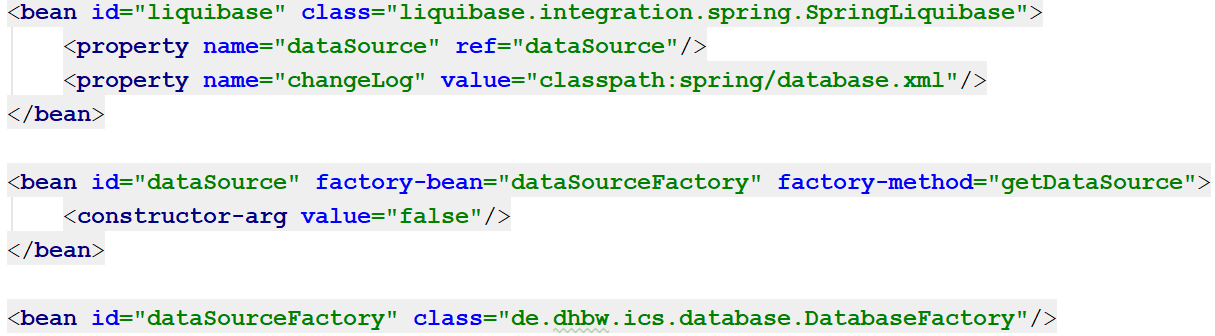
\includegraphics[width=\textwidth]{img/liquibase_beans}
	\captionsetup{format=hang}
	\caption[Spring-Konfiguration für Liquibase]{\label{fig:liquibase_spring}Spring-Konfiguration für Liquibase}
\end{figure}

Ein weiterer Vorteil von Liquibase ist, dass es eine Integration für das Spring-Framework, siehe Kapitel \ref{umsetzung:backend:grundgeruest}, mit sich bringt. Hierfür wurden mehrere Spring-Beans definiert, welche in Abbildung \ref{fig:liquibase_spring} zusehen sind. Wie man in dieser Abbildung erkennen kann, hängt das Bean für Liquibase (mit der \ac{ID} \glqq liquibase\grqq) von zwei Parametern ab. Der Parameter \glqq changelog\grqq \, gibt den Pfad zur Datei für die Konfiguration bzw. der Änderungshistorie an. Der zweite Parameter \glqq datasource\grqq \, hat als Übergabewert eine Referenz zu einem anderen Spring-Bean. Dieses Bean liefert ein \glqq DataSource\grqq-Objekt zurück welches in der Klasse \glqq DataSourceFactory.java\grqq erzeugt wird. Diese DataSource ist enthält die Verbindungsdaten für die Datenbankverbindung. Im aktuellen Release des \ac{ICS}-Projektes sind die Verbindungsdaten noch nicht parametrisiert, sondern fest im Code implementiert. Für einen späteren Auslieferungs-Release würden die Verbindungsdaten, wie URL, Passwort und Benutzername über Umgebungsvariablen setzbar sein.

Als Standard-Datenbank für die \ac{ICS}-Anwendung wurde eine H2-Datenbank verwendet. Die H2-Datenbank ist eine leichtgewichtige, in Java entwickelte Datenbank.\autocite{H2} Der Vorteil dieser ist, dass sie sehr einfach aufgebaut ist zur Laufzeit angelegt und bei bedarf auch in Memory erzeugt werden kann. Im Fall von \ac{ICS} wird eine H2-Datenbank beim erstem Starten der Anwendung in dem Ordner \glqq database\grqq, welcher sich in der Dateistruktur der Anwendung befindet. Dieser Ordner wird von dem im Kapitel \ref{umsetzung:backend:grundgeruest} erwähnten \glqq FileSystemInitializer\grqq \, erstellt, falls dieser noch nicht vorhanden ist.

\subsubsection{Anbindung an das Backend}

Um die einzelnen Entitäten der Datenbank im Backend zu verwirklichen, wurde ein zu dem Entwurfsmuster der Value-Objects ähnliches Verfahren angewandt. 

--> Anlehnung Domain Driven Development
--> 
--> 


\subsection{Fachkonzept}

\subsection{Restschnittstellen}

	
	\section[Frontend]{Frontend {\hfill \normalsize Jonas Dutzi, Dennis Köhler}}
	
	\subsection{Responsive Merkmale}
	Ziel des Projektes sollte es ebenfalls sein die Kinowebseite nicht nur für den großen Bildschirm am Computer zu entwickeln, sondern auch die Darstellung auf gegebenenfalls kleineren Endgeräten zu beachten. Die Nutzung von Websites auf mobilen Geräten steigt seit einigen Jahren kontinuierlich an. Im Jahr 2018 wurden zum Beispiel 52,2\% aller Aufrufe von Webseiten von Smartphones durchgeführt, während im Jahr 2009 noch nicht einmal 1\% aller Aufrufe durch die mobilen Geräte abgedeckt war\footnote{https://www.statista.com/statistics/241462/global-mobile-phone-website-traffic-share/}. Das zeigt auf wie wichtig das Thema des Responsive Webdesigns ist und welche Rolle es noch in der Zukunft spielen wird. Um diejenigen Nutzer, welche die Kinowebsite auch auf mobilen Endgeräten verwenden wollen nicht mit schlecht dargestelltem Inhalt zu enttäuschen, wurden in diesem Projekt hauptsächlich zwei Elemente des Bootstrap Frameworks zur Hilfe gezogen. Zum einen das Gitter System für die Anzeige von Inhalten und zum anderen die sich einklappende Navigationsleiste.
	
	Das in Bootstrap vorhandene Gitter System macht es möglich Inhalte, welche in Tabellenform bzw. in Reihen und Spalten, angezeigt werden an verschiedene Gerätegröße anzupassen. Hierfür werden drei vorgefertigte CSS-Klassen verwendet. Das äußere Div erhält die Klasse \texttt{.container} und umspannt den gesamten Inhalt. Innerhalb dieses Containers können Reihen und Spalten angelegt werden, welche durch weitere Divs mit den Klassen \texttt{.row} (Reihe) und \texttt{.col} (Spalte) realisiert werden. Diese kann man nach seinen Bedürfnissen schachteln, um die gewünschte Anzahl an Reihen und Spalten zu realisieren. Durch die Erweiterung \texttt{.col-\# (\# = 1-12)} kann die Breite und Anzahl der Elemente pro Reihe genau definiert werden. Hierbei stelle 12 die gesamte Seitenbreite dar, welche zum Beispiel mit einem 
	\texttt{col-12}  Element, zwei \texttt{col-6} Elementen oder drei \texttt{col-4} Elementen gefüllt werden kann. Um zu erreichen, dass bei variierender Gerätegröße unterschiedlich viele Elemente pro Reihe angezeigt werden, kann der Zusatz \texttt{.col-xx-\#}hinzugefügt werden. An stelle von xx kann nun eine vorgefertigten Gerätegrößen gewählt werden:
	
	\begin{table}[H]
		\centering
		\begin{tabular}{p{3,5cm} | c | c }
			\textbf{Klasse} & \textbf{Gerätegröße} & \textbf{Pixel} \\\toprule
			.col-xs-\# &  Extra small &  bis 576 \\
			.col-sm-\# &  Small &  bis 768  \\
			.col-md-\# &  Medium &  bis 922  \\
			.col-lg-\# &  Large &  bis 1200  \\
			.col-xl-\# &  Extra large &  über 1200  \\
		\end{tabular}
		\caption[Gerätegrößen]{\label{tab:gerätegrößen}Gerätegrößen }
	\end{table}
	
	Das Spalten-Div kann zu jeder Größe eine eigene Klasse mit definierter Breite implementieren. Am Beispiel der Filmkacheln der Startseite wird die Verwendung deutlich:
		\begin{center}
			<div class=“col-sm-12 col-md-6 col-lg-4”>
		\end{center}

	Bei kleinen Geräten wird die volle Breite (12) ausgenutzt und eine Kachel nimmt die gesamte Reihe ein. Übersteigt die Gerätegröße 768px teilen sich zwei Kacheln die volle Breite (6+6), ab 922px werden drei Kacheln nebeneinander angezeigt (4+4+4).
	
	Ein weiteres sich anpassendes Element stellt die Navigationsleiste dar. Ziel ist es bei kleineren Gerätegröße nicht den gesamten Inhalt anzuzeigen, sondern ihn hinter einem Button zu verstecken. Bei Betätigung dieses Buttons soll der Inhalt in Form einer Dropdown-Liste angezeigt werden. Um dies zu erreichen ist innerhalb des \texttt{<nav> </nav>} - HTML-Tags ein Button zu erstellen, welchem die in Bootstrap vorgefertigte CSS-Klasse \texttt{.navbar-toggler} zugewiesen wird. Die einzuklappenden Inhalte werden Innerhalb eines Divs, welches die vorgefertigten Klassen \texttt{.collapse}, \texttt{.navbar-collapse}, sowie eine feste ID besitzt, definiert. Diese ID wird dann dem Button-Attribut \texttt{data-target} zugewiesen. Zuletzt wird über die Klasse \texttt{.navbar-\\expand-lg} definiert, dass die Navigationsleiste ab einer Fenster-/Gerätebreite von kleiner als 992 Pixel hinter dem Button verschwindet. Die Abbildungen \vref{fig:navLeiste} und \vref{fig:navLeisteAus} zeigen das Ergebnis:
	\begin{figure}[H]
		\centering 
		
\includegraphics[width=13cm]{img/navLeiste.png}
		\captionsetup{format=hang}
		\caption[Navigationsleiste]{\label{fig:navLeiste} Navigationsleiste auf Geräten\\ mit einer Breite von über 992 Pixeln}
	\end{figure}
	
	\begin{figure}[H]
		\centering 
		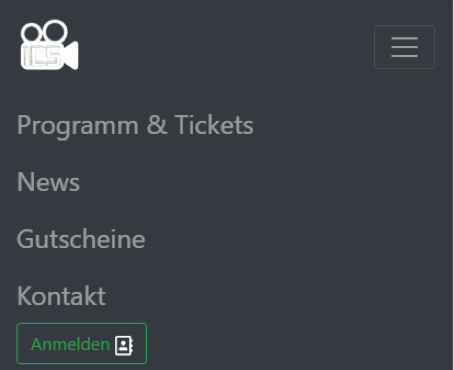
\includegraphics[width=6cm]{img/navLeisteAus.png}
		\captionsetup{format=hang}
		\caption[Navigationsleiste ausgeklappt]{\label{fig:navLeisteAus} Navigationsleiste ausgeklappt auf dem Smartphone (Breite 414 Pixel)}
	\end{figure}

	\subsection{Design}
	Um Nutzer anzuziehen und deren Erwartungen an eine moderne Website gerecht zu werden sollte das Ergebnis nicht nur funktional und responsive sein, sondern auch gut aussehen. Hierfür wurde bereits im Vorfeld der Umsetzung ein Design Entwurf angefertigt (Kapitel \vref{design}), welcher die Struktur vorgeben sollte. Diese wurde bei der Entwicklung auch weitestgehend eingehalten und es fanden neben der Umgestaltung der Navigationsleiste hauptsächlich kleinere Veränderungen, wie die Verschiebung von Inhalten statt. Einige Merkmale wurden im Entwurf jedoch noch nicht aufgeführt bzw. berücksichtigt und wurden erst während des Entwicklungsprozesses entschieden. 
	
	
	Einen wichtigen Punkt hierbei stellt die Farbwahl dar. Aufgrund der großen Beliebtheit, die die sogenannten \enquote{Darkmodes} neuer Betriebssystemversionen, Webseiten oder Apps mit sich bringen wurde auch für die Kinowebseite ein eher dunkleres Farbschema gewählt. Diese haben neben der subjektiven Einschätzung der Nutzer auch technische Vorteile wie die Entlastung der Augen in dunkleren Umgebungen oder geringeren Energieverbräuchen auf Endgeräten mit OLED-Display\footnote{https://www.futurezone.de/produkte/article215761243/Deshalb-bist-du-als-Android-User-mit-dem-Dark-Mode-im-Vorteil.html}. Um die Website einheitlich und nicht zu bunt zu gestalten wurde Grün als Akzentfarbe gewählt.
	
	
	Weitere unterschiede zum Entwurf sind in der Navigationsleiste erkennbar. Der Entwurf sieht eine zweizeilige Leiste mit getrennten, als Button gestalteten Schaltflächen vor. Bei der Betrachtung anderer Webseiten fiel jedoch auf, dass zum einen zweispaltige Navigationsleisten eher vermieden werden und zum anderen fließende Übergänge zwischen den Inhalten moderner wirken als durch Linien getrennte Bereiche. In Folge dessen wurde die Navigationsleiste in der \ac{ICS}-Webseite einzeilig und als ein zusammenhängender Bereich implementiert. Das Hervorheben der Schaltflächen geschieht durch die farbliche Aufhellung der entsprechenden Überschrift. 
	
	
	Das Hervorheben von Inhalten geschieht über die Webseite verteilt jedoch auf verschiedene Arten. Neben der erwähnten Aufhellung, kommen verschiedene Mauszeiger (Cursor) zum Einsatz. Den in HTML definierten Bereichen kann mithilfe des Cursor Attributs ein geeignetes Aussehen für den Mauszeiger zugeordnet werden. Inhalte die einen Link darstellen werden typischerweise mit dem \texttt{pointer}-Cursor versehen, welcher eine zeigende Hand symbolisiert. Neben diesem findet zum Beispiel der \texttt{not-allowed}-Cursor bei bereits belegten Sitzen des Sitzplans Verwendung. Eine weitere Möglichkeit des Hervorhebens ist bei den Filmkarten auf der Startseite verwendet worden. Diese beginnen bei Berührung des Cursors eine kleine Animation, welche durch ein JS-Script realisiert wurde und die gesamte Karte nach oben hebt. 
	
	Ein weiteres Designelement stellt der Slider dar. Dieser könnte beim Einsatz für ein Kino neben aktuellen Filmen auch Angebote oder spezielle Events werben. Auch wenn Kritiker Slider als nebensächlichen oder platzverschwendenden Inhalt ansehen und Studien die Ineffektivität der erreichten Werbewirkung darstellen\footnote{https://www.contentconsultants.de/blog/webdesign-slider-sind-out-weg-damit/} wurde sich bewusst dafür entschieden. Hierzu trugen die subjektiven Einschätzungen der Entwickler sowie der Ist-Vergleich zu anderen Kinowebseiten, siehe Kapitel \vref{istAnalyse}, bei.
	
	Zuletzt ist noch der Sitzplan zu erwähnen. Dieser wurde mithilfe des in %TODO 6.3.1 
	beschriebenen Frameworks erstellt und soll die Auswahl der zu reservierenden Sitze möglichst einfach und intuitiv gestalten. Der Saal wird als Menge von kleinen Quadraten, welche die Sitze darstellen, angezeigt. Bereits reservierte Sitze werden transparent grau, freie Sitze in grün eingefärbt. Der Nutzer kann die gewünschten Plätze durch Anklicken auswählen und gegebenenfalls durch erneutes Klicken abwählen. Abbildung \vref{fig:sitzplan} zeigt den Sitzplan in der finalen Version.
	
	\begin{figure}[H]
		\centering 
		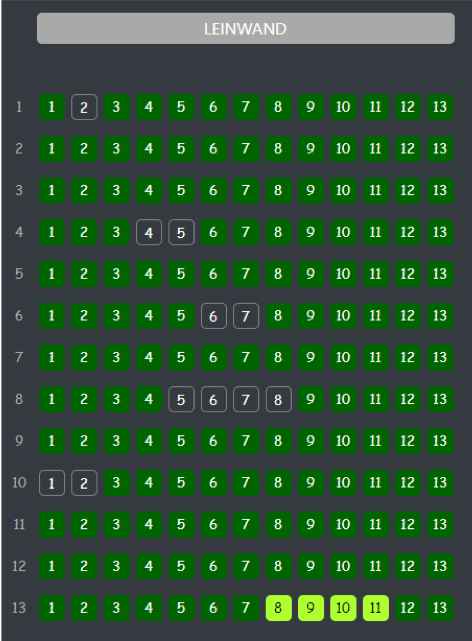
\includegraphics[width=9cm]{img/sitzplan.png}
		\captionsetup{format=hang}
		\caption[Sitzplan]{\label{fig:sitzplan} Sitzplan (Ausgewählte Sitze: 8,9,10,11 in Reihe 13)}
	\end{figure}

	\subsection{Ablauf des Bestellvorgangs}
	
	
	\section[Verknüpfung Back- und Frontend]{Verknüpfung Back- und Frontend {\hfill \normalsize Sandra Keller}}
	REST

	
	\section[Modultests]{Modultests{\hfill \normalsize Fabio Westphal}}
	Das Testen von Code stellt einen essenziellen Teil der Entwicklung von Software dar. Der ANSI/IEEE Standard 610.12-1990 definiert Tests folgendermaßen:	\enquote {An activity in which a system or component is executed under specified conditions, the results are observed or recorded, and an evaluation is made of some aspect of the system or component.} Man unterscheidet grundsätzlich Whitebox- und Blackbox-Tests. Bei Whitebox-Tests wird die innere Funktionsweise der Software getestet, wohingegen bei Blackbox-Tests kein Wissen über den Quellcode zugrundeliegt und nur der geforderte Funktionsumfang getestet wird.\autocite{franz2007handbuch}[Vgl.][S.28] Im Projekt wurden hauptsächlich Komponententests angewendet, welche zu den Whitebox-Tests zählen. Hierbei werden Klassen und Methoden einzeln parallel zur weiteren Entwicklung getestet. Durch die kleinschrittige Testweise tragen sie auch zur lebenden Dokumentation bei. Wichtig ist dabei, dass jeder Test korrekt,
schnell, abgeschlossen,	isoliert, sprechend benannt, wartbar und einfach durchführbar
ist.
	Es muss der gesamte Code einmal durchlaufen werden, um maximale Korrektheit zu sichern.\autocite{witte2015testmanagement}[Vgl.][S.50] Bei überschauberen Systemen kann man aber auch nur kritische Teile testen. Um die Tests automatisiert auszuführen, werden Test-Frameworks verwendet. In diesem Projekt wird das bekannte Framework JUnit benutzt.
	Bei Datenbankzugriffsklassen ist es vor allem wichtig, die \ac{CRUD}-Operationen zu testen. Diese gelten als die essenziellen Funktionen, wenn es um den Zugriff auf Datenbanken geht. Im Projekt wurde dafür die Klasse \texttt{DaoTestHelper} verwendet, die entsprechende Schnittstellen für die Testklassen zur Verfügung stellt. Im Zuge eines Tests werden zunächst Beispielobjekte erzeugt und persistiert. Anschließend werden die Grundoperationen mithilfe der Helper-Klasse getestet. Am Beispiel der Klasse \texttt{MovieDaoTest} sieht das wie folgt aus:
	\begin{lstlisting}
public class MovieDaoTest {

	private static Movie movie;
	private static Genre genre;
	
	@Autowired
	private GenreDao genreDao;
	
	@Autowired
	private MovieDao movieDao;
	
	@BeforeClass
	public static void setUp() throws Exception {
		movie = new Movie(2015, "TestMovie", "Nice Test Movie", 12, 120);
		genre = new Genre("testGenre");
		movie.setGenre(genre);
	}
	
	@Test
	public void test1Persist() {
		assertFalse(this.movieDao.persist(movie));
		assertTrue(this.genreDao.persist(genre));
		DaoTestHelper.persist(this.movieDao, movie);
	}
	
	@Test
	public void test2Get() {
		DaoTestHelper.get(this.movieDao, movie, movie.getUuid());
	}
	
	@Test
	public void test3GetAll() {
		DaoTestHelper.getAll(this.movieDao, movie);
	}
	
	@Test
	public void test4Update() {
		Movie testMovie = new Movie(movie.getUuid(), 2000,"updatedMovie", movie.getDescription(), movie.getFsk(), movie.getRunTime());
		testMovie.setGenre(movie.getGenre());
		DaoTestHelper.update(this.movieDao, movie.getUuid(), movie, testMovie);
	}
	
	@Test
	public void test5Delete() {
		DaoTestHelper.delete(this.movieDao, movie.getUuid());
	}
}
	\end{lstlisting}
	Beim Ausführen der Tests gibt es in der Entwicklungsumgebung IntelliJ die Möglichkeit, die Abdeckung zu berechnen. Dabei werden zum einen die Zeilen gezählt, die von den Tests betroffen sind und zum anderen die Methoden bzw. Klassen. In Relation zur Gesamtheit der Zeilen - bzw. Methoden oder Klassen - ergibt dies die Testabdeckung als Prozentzahl (siehe Abb. \ref{fig:TestCoverage}).\newline
	\begin{figure} 
		\centering 
		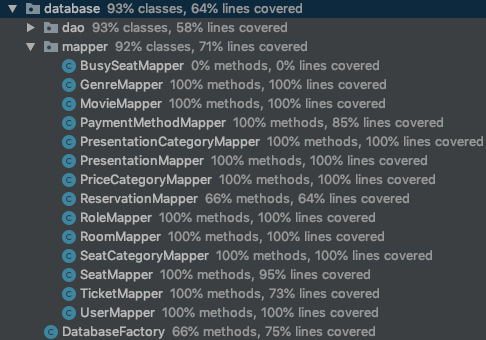
\includegraphics[scale=0.6]{img/testCoverage.png}
		\captionsetup{format=hang}
		\centering\caption[Testabdeckung]{\label{fig:TestCoverage} Übersicht der Testabdeckung}
	\end{figure}
	Die Testabdeckung ist häufig ein faktisches Kriterium für die Qualität des Codes bei Abnahme des Projekts. Beim Erreichen einer bestimmten Prozentzahl fällt allerdings auf, dass diese beim Schreiben der Tests nicht linear steigt. Das liegt daran, dass viele Klassen, die explizit getestet werden, Methoden anderer Klassen wie beispielsweise Superklassen oder Helper-Klassen nutzen. Somit werden diese direkt auch getestet. Andere Klassen wiederum verwenden genau die gleiche Superklasse (oder Helper-Klasse...), die bereits zuvor fremdgetestet wurde. Es sind also weniger Zeilen Code, die für die Testabdeckung zählen, obwohl ähnlich viele Zeilen durchlaufen werden. Daher ist es in der Regel der Fall, dass bei den ersten Tests die Testabdeckung stark wächst, dann jedoch immer langsamer.
	
	
	\section[Ausblick]{Ausblick {\hfill \normalsize Milena Zahn}}\label{Ausblick}
	%\subsection{Lessons Learned} 
	Die Bereiche, an denen gearbeitet wurde, waren vielfältig. Zuerst waren alle an der Analyse sowie der Erarbeitung des Entwurfs beteiligt. Dann musste sich das Team erarbeiten, wie ein solches Projekt umgesetzt werden kann. Die Programmierung des Backends war für einige der Teammitglieder komplett neu, aber da das Team sehr unterschiedliche Fähigkeiten besitzt, war dies in der geplanten Projektzeit möglich. Auch die Erstellung des Frontends war eine interessante Erfahrung. Die Verbindung von diesem mit dem Backend war für die meisten von uns eine weitere Herausforderung, da in diesem Bereich noch wenige Erfahrungen gemacht wurden. 
	Neben dem technischen Wissen haben die Teammitglieder auch einige weitere Kompetenzen in dem Projekt erworben. Eine davon ist, dass es sehr wichtig ist, andere Projekte, an denen die Teammitglieder außerhalb des Moduls arbeiten müssen, bei dem Projektplans zu berücksichtigen. Obwohl dies sehr schwierig ist, kann dies helfen, den Projektplan genauer und realistischer zu erstellen. Es ist sehr wichtig, für jede Aufgabe genügend Zeit einzuplanen, um unerwartete Herausforderungen zu bewältigen. Die selbständige Erarbeitung von Vorgehensweisen und Lösungskonzepte ist eine weitere in diesem Projekt erworbene Kompetenz.
	Eine weitere Hürde war die Gruppengröße von acht Personen. Es ist schwierig das Potenzial der Gruppe voll ausschöpfen, weil die Arbeit innerhalb der Gruppe gut organisiert werden muss.  Um eine übermäßige Koordination der Mitglieder und lange Kommunikationswege zu vermeiden, haben wir die Gruppe in Untergruppen mit verschiedenen Aufgabenbereichen aufgeteilt. Somit konnte eine schnelle Entscheidungsfindung und kurzfristige Absprachen garantiert werden. Insgesamt wurden in der engen Projektzeit viele unterschiedliche Kompetenzen erworben und vor allem die theoretischen Inhalte der Vorlesung Systemanalyse angewandt.
	